\documentclass[twoside]{book}

% Packages required by doxygen
\usepackage{fixltx2e}
\usepackage{calc}
\usepackage{doxygen}
\usepackage[export]{adjustbox} % also loads graphicx
\usepackage{graphicx}
\usepackage[utf8]{inputenc}
\usepackage{makeidx}
\usepackage{multicol}
\usepackage{multirow}
\PassOptionsToPackage{warn}{textcomp}
\usepackage{textcomp}
\usepackage[nointegrals]{wasysym}
\usepackage[table]{xcolor}

% NLS support packages
\usepackage[T2A]{fontenc}
\usepackage[russian]{babel}

% Font selection
\usepackage[T1]{fontenc}
\usepackage[scaled=.90]{helvet}
\usepackage{courier}
\usepackage{amssymb}
\usepackage{sectsty}
\renewcommand{\familydefault}{\sfdefault}
\allsectionsfont{%
  \fontseries{bc}\selectfont%
  \color{darkgray}%
}
\renewcommand{\DoxyLabelFont}{%
  \fontseries{bc}\selectfont%
  \color{darkgray}%
}
\newcommand{\+}{\discretionary{\mbox{\scriptsize$\hookleftarrow$}}{}{}}

% Page & text layout
\usepackage{geometry}
\geometry{%
  a4paper,%
  top=2.5cm,%
  bottom=2.5cm,%
  left=2.5cm,%
  right=2.5cm%
}
\tolerance=750
\hfuzz=15pt
\hbadness=750
\setlength{\emergencystretch}{15pt}
\setlength{\parindent}{0cm}
\setlength{\parskip}{3ex plus 2ex minus 2ex}
\makeatletter
\renewcommand{\paragraph}{%
  \@startsection{paragraph}{4}{0ex}{-1.0ex}{1.0ex}{%
    \normalfont\normalsize\bfseries\SS@parafont%
  }%
}
\renewcommand{\subparagraph}{%
  \@startsection{subparagraph}{5}{0ex}{-1.0ex}{1.0ex}{%
    \normalfont\normalsize\bfseries\SS@subparafont%
  }%
}
\makeatother

% Headers & footers
\usepackage{fancyhdr}
\pagestyle{fancyplain}
\fancyhead[LE]{\fancyplain{}{\bfseries\thepage}}
\fancyhead[CE]{\fancyplain{}{}}
\fancyhead[RE]{\fancyplain{}{\bfseries\leftmark}}
\fancyhead[LO]{\fancyplain{}{\bfseries\rightmark}}
\fancyhead[CO]{\fancyplain{}{}}
\fancyhead[RO]{\fancyplain{}{\bfseries\thepage}}
\fancyfoot[LE]{\fancyplain{}{}}
\fancyfoot[CE]{\fancyplain{}{}}
\fancyfoot[RE]{\fancyplain{}{\bfseries\scriptsize Создано системой Doxygen }}
\fancyfoot[LO]{\fancyplain{}{\bfseries\scriptsize Создано системой Doxygen }}
\fancyfoot[CO]{\fancyplain{}{}}
\fancyfoot[RO]{\fancyplain{}{}}
\renewcommand{\footrulewidth}{0.4pt}
\renewcommand{\chaptermark}[1]{%
  \markboth{#1}{}%
}
\renewcommand{\sectionmark}[1]{%
  \markright{\thesection\ #1}%
}

% Indices & bibliography
\usepackage{natbib}
\usepackage[titles]{tocloft}
\setcounter{tocdepth}{3}
\setcounter{secnumdepth}{5}
\makeindex

% Hyperlinks (required, but should be loaded last)
\usepackage{ifpdf}
\ifpdf
  \usepackage[pdftex,pagebackref=true]{hyperref}
\else
  \usepackage[ps2pdf,pagebackref=true]{hyperref}
\fi
\hypersetup{%
  colorlinks=true,%
  linkcolor=blue,%
  citecolor=blue,%
  unicode%
}

% Custom commands
\newcommand{\clearemptydoublepage}{%
  \newpage{\pagestyle{empty}\cleardoublepage}%
}

\usepackage{caption}
\captionsetup{labelsep=space,justification=centering,font={bf},singlelinecheck=off,skip=4pt,position=top}

%===== C O N T E N T S =====

\begin{document}

% Titlepage & ToC
\hypersetup{pageanchor=false,
             bookmarksnumbered=true,
             pdfencoding=unicode
            }
\pagenumbering{alph}
\begin{titlepage}
\vspace*{7cm}
\begin{center}%
{\Large Toxic-\/\+Comment-\/\+Classification }\\
\vspace*{1cm}
{\large Создано системой Doxygen 1.8.14}\\
\end{center}
\end{titlepage}
\clearemptydoublepage
\pagenumbering{roman}
\tableofcontents
\clearemptydoublepage
\pagenumbering{arabic}
\hypersetup{pageanchor=true}

%--- Begin generated contents ---
\chapter{Алфавитный указатель пространств имен}
\section{Пространства имен}
Полный список документированных пространств имен.\begin{DoxyCompactList}
\item\contentsline{section}{\mbox{\hyperlink{namespacetcc}{tcc}} \\*Пространство имен tcc }{\pageref{namespacetcc}}{}
\end{DoxyCompactList}

\chapter{Иерархический список классов}
\section{Иерархия классов}
Иерархия классов.\begin{DoxyCompactList}
\item \contentsline{section}{Controller}{\pageref{class_controller}}{}
\begin{DoxyCompactList}
\item \contentsline{section}{Main\+Controller}{\pageref{class_main_controller}}{}
\end{DoxyCompactList}
\item \contentsline{section}{Core}{\pageref{class_core}}{}
\item \contentsline{section}{Data\+Processing}{\pageref{class_data_processing}}{}
\item \contentsline{section}{Data\+Provider}{\pageref{class_data_provider}}{}
\begin{DoxyCompactList}
\item \contentsline{section}{File\+Data\+Provider}{\pageref{class_file_data_provider}}{}
\end{DoxyCompactList}
\item \contentsline{section}{Message}{\pageref{class_message}}{}
\end{DoxyCompactList}

\chapter{Алфавитный указатель классов}
\section{Классы}
Классы с их кратким описанием.\begin{DoxyCompactList}
\item\contentsline{section}{\mbox{\hyperlink{class_controller}{Controller}} \\*Интерфейс для классов контроллеров управляющими ходом программы }{\pageref{class_controller}}{}
\item\contentsline{section}{\mbox{\hyperlink{class_core}{Core}} \\*Интерфейс классов ядра для определения \char`\"{}недоброжелательности\char`\"{} текста }{\pageref{class_core}}{}
\item\contentsline{section}{\mbox{\hyperlink{class_data_processing}{Data\+Processing}} \\*Интерфейс для классов предобработки текста }{\pageref{class_data_processing}}{}
\item\contentsline{section}{\mbox{\hyperlink{class_data_provider}{Data\+Provider}} \\*Интерфейс для классов считывания/записи данных }{\pageref{class_data_provider}}{}
\item\contentsline{section}{\mbox{\hyperlink{class_file_data_provider}{File\+Data\+Provider}} \\*Класс для считывания/записи данных из/в файл(а) }{\pageref{class_file_data_provider}}{}
\item\contentsline{section}{\mbox{\hyperlink{class_main_controller}{Main\+Controller}} \\*Основной класс контроллер управляющий ходом программы }{\pageref{class_main_controller}}{}
\item\contentsline{section}{\mbox{\hyperlink{class_message}{Message}} }{\pageref{class_message}}{}
\end{DoxyCompactList}

\chapter{Пространства имен}
\hypertarget{namespacetcc}{}\section{Пространство имен tcc}
\label{namespacetcc}\index{tcc@{tcc}}


Пространство имен tcc.  


\subsection*{Классы}
\begin{DoxyCompactItemize}
\item 
class \mbox{\hyperlink{classtcc_1_1_controller}{Controller}}
\begin{DoxyCompactList}\small\item\em Интерфейс для классов контроллеров управляющими ходом программы \end{DoxyCompactList}\item 
class \mbox{\hyperlink{classtcc_1_1_core}{Core}}
\begin{DoxyCompactList}\small\item\em Интерфейс классов ядра для классификации \char`\"{}недоброжелательности\char`\"{} текста \end{DoxyCompactList}\item 
class \mbox{\hyperlink{classtcc_1_1_data_processing}{Data\+Processing}}
\begin{DoxyCompactList}\small\item\em Интерфейс для классов предобработки текста \end{DoxyCompactList}\item 
class \mbox{\hyperlink{classtcc_1_1_data_provider}{Data\+Provider}}
\begin{DoxyCompactList}\small\item\em Интерфейс для классов считывания/записи данных \end{DoxyCompactList}\item 
class \mbox{\hyperlink{classtcc_1_1_file_data_provider}{File\+Data\+Provider}}
\begin{DoxyCompactList}\small\item\em Класс для считывания/записи данных из/в файл(а) \end{DoxyCompactList}\item 
class \mbox{\hyperlink{classtcc_1_1_main_controller}{Main\+Controller}}
\begin{DoxyCompactList}\small\item\em Основной класс контроллер управляющий ходом программы \end{DoxyCompactList}\item 
class \mbox{\hyperlink{classtcc_1_1_message}{Message}}
\item 
class \mbox{\hyperlink{classtcc_1_1_random_core}{Random\+Core}}
\begin{DoxyCompactList}\small\item\em Класс -\/ ядро для классификации \char`\"{}недоброжелательности\char`\"{} текста \end{DoxyCompactList}\end{DoxyCompactItemize}


\subsection{Подробное описание}
Пространство имен tcc. 

namespace tcc 
\chapter{Классы}
\hypertarget{classtcc_1_1_controller}{}\section{tcc\+:\+:Controller Class Reference}
\label{classtcc_1_1_controller}\index{tcc\+::\+Controller@{tcc\+::\+Controller}}


Основной класс контроллер управляющий ходом программы  




{\ttfamily \#include $<$Controller.\+h$>$}

\subsection*{Public Member Functions}
\begin{DoxyCompactItemize}
\item 
\hyperlink{classtcc_1_1_controller_addf3fea20133594d55a03f5134614b98}{Controller} (std\+::shared\+\_\+ptr$<$ \hyperlink{classtcc_1_1_data_provider}{Data\+Provider} $>$ data\+\_\+provider)
\begin{DoxyCompactList}\small\item\em Конструктор класса \end{DoxyCompactList}\item 
void \hyperlink{classtcc_1_1_controller_a61233522bd4c1a17dddb76f7f337bf3a}{init} ()\hypertarget{classtcc_1_1_controller_a61233522bd4c1a17dddb76f7f337bf3a}{}\label{classtcc_1_1_controller_a61233522bd4c1a17dddb76f7f337bf3a}

\begin{DoxyCompactList}\small\item\em Инициализация классификатора \end{DoxyCompactList}\item 
void \hyperlink{classtcc_1_1_controller_a41b047e081c2ae0350379b5d84e5d2a3}{run} (\hyperlink{namespacetcc_a9bdf9e81347b7904a6a7f8427d6465dc}{text\+Vec} \&texts)\hypertarget{classtcc_1_1_controller_a41b047e081c2ae0350379b5d84e5d2a3}{}\label{classtcc_1_1_controller_a41b047e081c2ae0350379b5d84e5d2a3}

\begin{DoxyCompactList}\small\item\em Обработка текста \end{DoxyCompactList}\item 
void \hyperlink{classtcc_1_1_controller_a957db61db1243fb15d8de927bfa90388}{save} ()\hypertarget{classtcc_1_1_controller_a957db61db1243fb15d8de927bfa90388}{}\label{classtcc_1_1_controller_a957db61db1243fb15d8de927bfa90388}

\begin{DoxyCompactList}\small\item\em Сохранить текущий результат \end{DoxyCompactList}\item 
void \hyperlink{classtcc_1_1_controller_a76359375dbebe6f184120f201c9b8821}{close} ()\hypertarget{classtcc_1_1_controller_a76359375dbebe6f184120f201c9b8821}{}\label{classtcc_1_1_controller_a76359375dbebe6f184120f201c9b8821}

\begin{DoxyCompactList}\small\item\em сохранить то, что осталось в буфере перед выыходом \end{DoxyCompactList}\end{DoxyCompactItemize}


\subsection{Detailed Description}
Основной класс контроллер управляющий ходом программы 

\subsection{Constructor \& Destructor Documentation}
\index{tcc\+::\+Controller@{tcc\+::\+Controller}!Controller@{Controller}}
\index{Controller@{Controller}!tcc\+::\+Controller@{tcc\+::\+Controller}}
\subsubsection[{\texorpdfstring{Controller(std\+::shared\+\_\+ptr$<$ Data\+Provider $>$ data\+\_\+provider)}{Controller(std::shared_ptr< DataProvider > data_provider)}}]{\setlength{\rightskip}{0pt plus 5cm}tcc\+::\+Controller\+::\+Controller (
\begin{DoxyParamCaption}
\item[{std\+::shared\+\_\+ptr$<$ {\bf Data\+Provider} $>$}]{data\+\_\+provider}
\end{DoxyParamCaption}
)\hspace{0.3cm}{\ttfamily [inline]}}\hypertarget{classtcc_1_1_controller_addf3fea20133594d55a03f5134614b98}{}\label{classtcc_1_1_controller_addf3fea20133594d55a03f5134614b98}


Конструктор класса 


\begin{DoxyParams}{Parameters}
{\em data\+\_\+provider} & Указатель на используемый провайдер \\
\hline
\end{DoxyParams}


The documentation for this class was generated from the following file\+:\begin{DoxyCompactItemize}
\item 
src/\+Controllers/Controller.\+h\end{DoxyCompactItemize}

\hypertarget{classtcc_1_1_core}{}\section{Класс tcc\+:\+:Core}
\label{classtcc_1_1_core}\index{tcc\+::\+Core@{tcc\+::\+Core}}


Интерфейс классов ядра для классификации \char`\"{}недоброжелательности\char`\"{} текста  




{\ttfamily \#include $<$Core.\+h$>$}

Граф наследования\+:tcc\+:\+:Core\+:\begin{figure}[H]
\begin{center}
\leavevmode
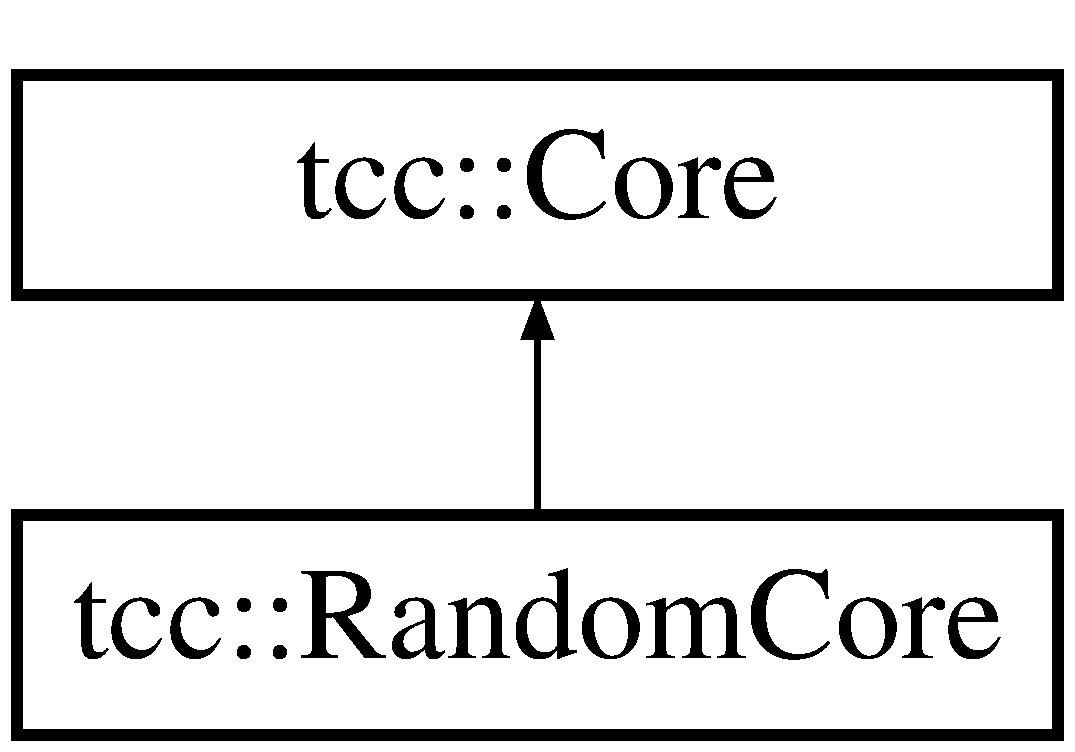
\includegraphics[height=2.000000cm]{classtcc_1_1_core}
\end{center}
\end{figure}


\subsection{Подробное описание}
Интерфейс классов ядра для классификации \char`\"{}недоброжелательности\char`\"{} текста 

См. определение в файле Core.\+h строка 14



Объявления и описания членов класса находятся в файле\+:\begin{DoxyCompactItemize}
\item 
Cores/Core.\+h\end{DoxyCompactItemize}

\hypertarget{classtcc_1_1_data_processing}{}\section{Класс tcc\+:\+:Data\+Processing}
\label{classtcc_1_1_data_processing}\index{tcc\+::\+Data\+Processing@{tcc\+::\+Data\+Processing}}


Интерфейс для классов предобработки текста  




{\ttfamily \#include $<$Data\+Handler.\+h$>$}



\subsection{Подробное описание}
Интерфейс для классов предобработки текста 

См. определение в файле Data\+Handler.\+h строка 14



Объявления и описания членов класса находятся в файле\+:\begin{DoxyCompactItemize}
\item 
Data\+Handlers/Data\+Handler.\+h\end{DoxyCompactItemize}

\hypertarget{classtcc_1_1_data_provider}{}\section{tcc\+:\+:Data\+Provider Class Reference}
\label{classtcc_1_1_data_provider}\index{tcc\+::\+Data\+Provider@{tcc\+::\+Data\+Provider}}


Интерфейс для классов считывания/записи данных  




{\ttfamily \#include $<$Data\+Provider.\+h$>$}

Inheritance diagram for tcc\+:\+:Data\+Provider\+:\begin{figure}[H]
\begin{center}
\leavevmode
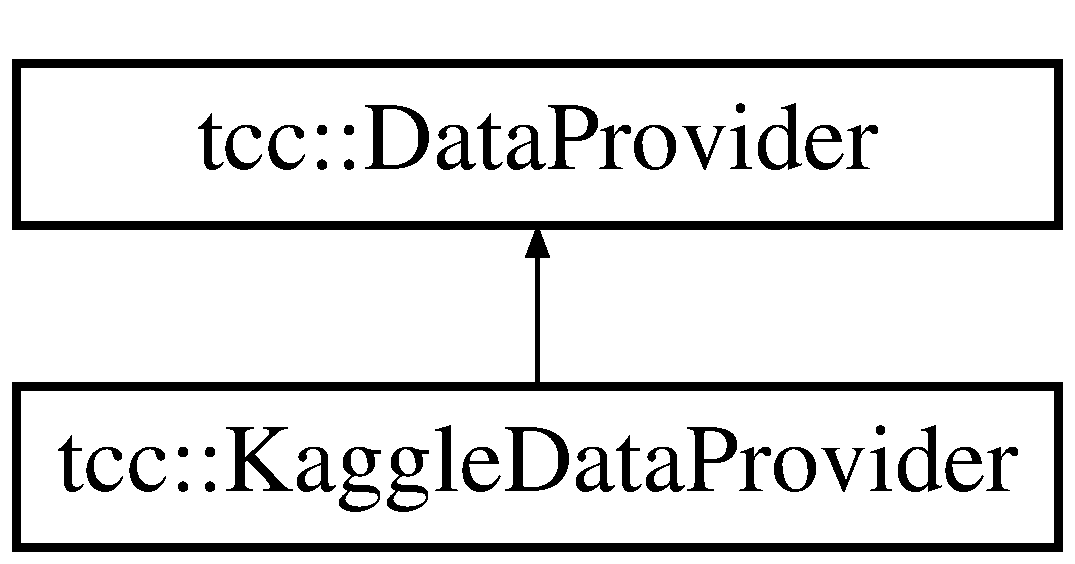
\includegraphics[height=2.000000cm]{classtcc_1_1_data_provider}
\end{center}
\end{figure}
\subsection*{Public Member Functions}
\begin{DoxyCompactItemize}
\item 
virtual std\+::vector$<$ json $>$ \hyperlink{classtcc_1_1_data_provider_af5a33d2b9d234e39547a148b8f99cf6f}{get\+\_\+data} () const  =0
\begin{DoxyCompactList}\small\item\em Виртуальная функция для считывания данных \end{DoxyCompactList}\end{DoxyCompactItemize}


\subsection{Detailed Description}
Интерфейс для классов считывания/записи данных 

\subsection{Member Function Documentation}
\index{tcc\+::\+Data\+Provider@{tcc\+::\+Data\+Provider}!get\+\_\+data@{get\+\_\+data}}
\index{get\+\_\+data@{get\+\_\+data}!tcc\+::\+Data\+Provider@{tcc\+::\+Data\+Provider}}
\subsubsection[{\texorpdfstring{get\+\_\+data() const  =0}{get_data() const  =0}}]{\setlength{\rightskip}{0pt plus 5cm}virtual std\+::vector$<$json$>$ tcc\+::\+Data\+Provider\+::get\+\_\+data (
\begin{DoxyParamCaption}
{}
\end{DoxyParamCaption}
) const\hspace{0.3cm}{\ttfamily [pure virtual]}}\hypertarget{classtcc_1_1_data_provider_af5a33d2b9d234e39547a148b8f99cf6f}{}\label{classtcc_1_1_data_provider_af5a33d2b9d234e39547a148b8f99cf6f}


Виртуальная функция для считывания данных 

\begin{DoxyReturn}{Returns}
Вектор структур данных, содержащих в себе считанные данные 
\end{DoxyReturn}

\begin{DoxyExceptions}{Exceptions}
{\em I\+O\+Exception} & Исключение возникающее при проблемах с чтением файла \\
\hline
\end{DoxyExceptions}


Implemented in \hyperlink{classtcc_1_1_kaggle_data_provider_a9a70415967019e9199957bf208a31478}{tcc\+::\+Kaggle\+Data\+Provider}.



The documentation for this class was generated from the following file\+:\begin{DoxyCompactItemize}
\item 
src/\+Data\+Providers/Data\+Provider.\+h\end{DoxyCompactItemize}

\hypertarget{classtcc_1_1_file_data_provider}{}\section{Класс tcc\+:\+:File\+Data\+Provider}
\label{classtcc_1_1_file_data_provider}\index{tcc\+::\+File\+Data\+Provider@{tcc\+::\+File\+Data\+Provider}}


Класс для считывания/записи данных из/в файл(а)  




{\ttfamily \#include $<$Data\+Provider.\+h$>$}

Граф наследования\+:tcc\+:\+:File\+Data\+Provider\+:\begin{figure}[H]
\begin{center}
\leavevmode
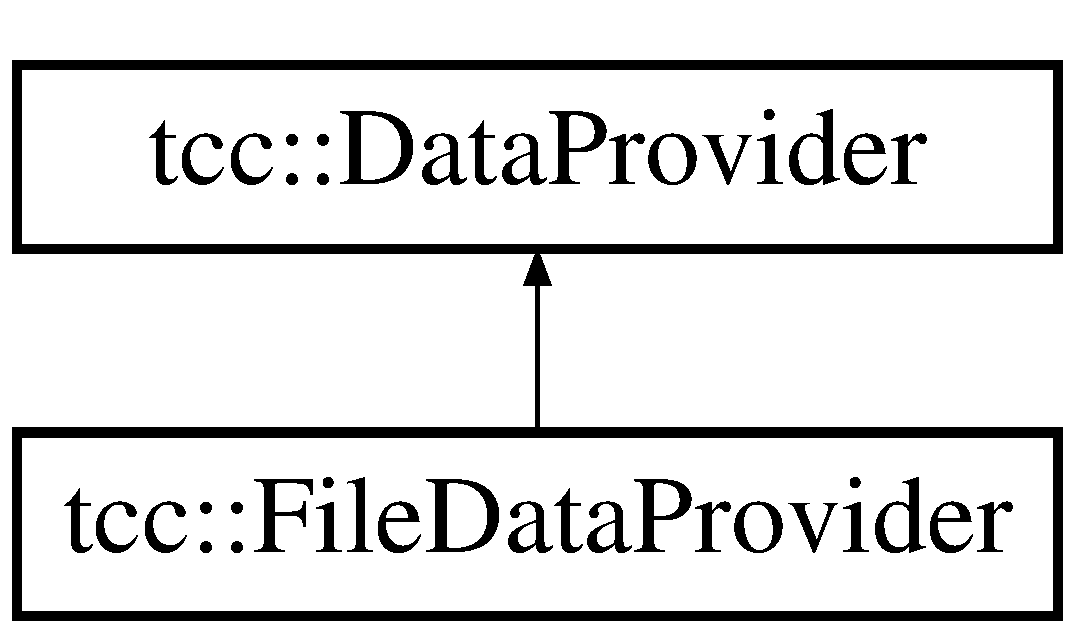
\includegraphics[height=2.000000cm]{classtcc_1_1_file_data_provider}
\end{center}
\end{figure}
\subsection*{Открытые члены}
\begin{DoxyCompactItemize}
\item 
\mbox{\hyperlink{classtcc_1_1_file_data_provider_a86089a313a91640e85c4eb6e221ec357}{File\+Data\+Provider}} (std\+::vector$<$ char $>$ input\+\_\+file, std\+::vector$<$ char $>$ output\+\_\+file)
\begin{DoxyCompactList}\small\item\em Конструктор класса \end{DoxyCompactList}\item 
std\+::vector$<$ \mbox{\hyperlink{classtcc_1_1_message}{Message}} $>$ \mbox{\hyperlink{classtcc_1_1_file_data_provider_ada1c8160929d1b3a2de366bda89ec0b8}{get\+\_\+data}} () const override
\begin{DoxyCompactList}\small\item\em Функция для считывания данных из файла \end{DoxyCompactList}\item 
bool \mbox{\hyperlink{classtcc_1_1_file_data_provider_a969360abf9313a4b81de0af227025fa0}{save\+\_\+data}} (const \mbox{\hyperlink{classtcc_1_1_message}{Message}} \&msg) const override
\begin{DoxyCompactList}\small\item\em Функция для записи данных в файл \end{DoxyCompactList}\end{DoxyCompactItemize}


\subsection{Подробное описание}
Класс для считывания/записи данных из/в файл(а) 

См. определение в файле Data\+Provider.\+h строка 35



\subsection{Конструктор(ы)}
\mbox{\Hypertarget{classtcc_1_1_file_data_provider_a86089a313a91640e85c4eb6e221ec357}\label{classtcc_1_1_file_data_provider_a86089a313a91640e85c4eb6e221ec357}} 
\index{tcc\+::\+File\+Data\+Provider@{tcc\+::\+File\+Data\+Provider}!File\+Data\+Provider@{File\+Data\+Provider}}
\index{File\+Data\+Provider@{File\+Data\+Provider}!tcc\+::\+File\+Data\+Provider@{tcc\+::\+File\+Data\+Provider}}
\subsubsection{\texorpdfstring{File\+Data\+Provider()}{FileDataProvider()}}
{\footnotesize\ttfamily tcc\+::\+File\+Data\+Provider\+::\+File\+Data\+Provider (\begin{DoxyParamCaption}\item[{std\+::vector$<$ char $>$}]{input\+\_\+file,  }\item[{std\+::vector$<$ char $>$}]{output\+\_\+file }\end{DoxyParamCaption})\hspace{0.3cm}{\ttfamily [inline]}}



Конструктор класса 


\begin{DoxyParams}{Аргументы}
{\em input\+\_\+file} & Имя файла для чтения \\
\hline
{\em output\+\_\+file} & Имя файла для записи \\
\hline
\end{DoxyParams}


См. определение в файле Data\+Provider.\+h строка 46



\subsection{Методы}
\mbox{\Hypertarget{classtcc_1_1_file_data_provider_ada1c8160929d1b3a2de366bda89ec0b8}\label{classtcc_1_1_file_data_provider_ada1c8160929d1b3a2de366bda89ec0b8}} 
\index{tcc\+::\+File\+Data\+Provider@{tcc\+::\+File\+Data\+Provider}!get\+\_\+data@{get\+\_\+data}}
\index{get\+\_\+data@{get\+\_\+data}!tcc\+::\+File\+Data\+Provider@{tcc\+::\+File\+Data\+Provider}}
\subsubsection{\texorpdfstring{get\+\_\+data()}{get\_data()}}
{\footnotesize\ttfamily std\+::vector$<$\mbox{\hyperlink{classtcc_1_1_message}{Message}}$>$ tcc\+::\+File\+Data\+Provider\+::get\+\_\+data (\begin{DoxyParamCaption}{ }\end{DoxyParamCaption}) const\hspace{0.3cm}{\ttfamily [override]}, {\ttfamily [virtual]}}



Функция для считывания данных из файла 

\begin{DoxyReturn}{Возвращает}
Вектор структур данных, содержащих в себе считанные данные 
\end{DoxyReturn}

\begin{DoxyExceptions}{Исключения}
{\em I\+O\+Exception} & Исключение возникающее при проблемах с чтением файла \\
\hline
\end{DoxyExceptions}


Замещает \mbox{\hyperlink{classtcc_1_1_data_provider}{tcc\+::\+Data\+Provider}}.

\mbox{\Hypertarget{classtcc_1_1_file_data_provider_a969360abf9313a4b81de0af227025fa0}\label{classtcc_1_1_file_data_provider_a969360abf9313a4b81de0af227025fa0}} 
\index{tcc\+::\+File\+Data\+Provider@{tcc\+::\+File\+Data\+Provider}!save\+\_\+data@{save\+\_\+data}}
\index{save\+\_\+data@{save\+\_\+data}!tcc\+::\+File\+Data\+Provider@{tcc\+::\+File\+Data\+Provider}}
\subsubsection{\texorpdfstring{save\+\_\+data()}{save\_data()}}
{\footnotesize\ttfamily bool tcc\+::\+File\+Data\+Provider\+::save\+\_\+data (\begin{DoxyParamCaption}\item[{const \mbox{\hyperlink{classtcc_1_1_message}{Message}} \&}]{msg }\end{DoxyParamCaption}) const\hspace{0.3cm}{\ttfamily [override]}, {\ttfamily [virtual]}}



Функция для записи данных в файл 


\begin{DoxyParams}{Аргументы}
{\em msg} & Структура данных, содержащая в себе данные подлежащие записи \\
\hline
\end{DoxyParams}
\begin{DoxyReturn}{Возвращает}
Булевое значение\+:
\begin{DoxyItemize}
\item 0 запись не удаласть
\item 1 запись удалась 
\end{DoxyItemize}
\end{DoxyReturn}


Замещает \mbox{\hyperlink{classtcc_1_1_data_provider}{tcc\+::\+Data\+Provider}}.



Объявления и описания членов класса находятся в файле\+:\begin{DoxyCompactItemize}
\item 
Data\+Providers/Data\+Provider.\+h\end{DoxyCompactItemize}

\hypertarget{classtcc_1_1_main_controller}{}\section{Класс tcc\+:\+:Main\+Controller}
\label{classtcc_1_1_main_controller}\index{tcc\+::\+Main\+Controller@{tcc\+::\+Main\+Controller}}


Основной класс контроллер управляющий ходом программы  




{\ttfamily \#include $<$Controller.\+h$>$}

Граф наследования\+:tcc\+:\+:Main\+Controller\+:\begin{figure}[H]
\begin{center}
\leavevmode
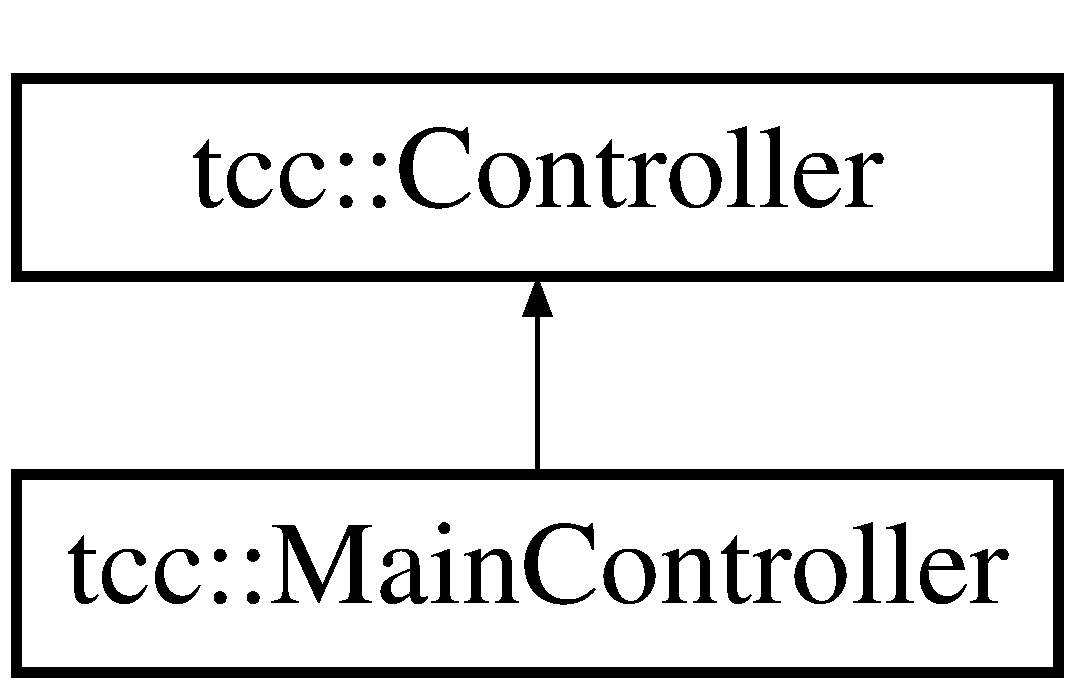
\includegraphics[height=2.000000cm]{classtcc_1_1_main_controller}
\end{center}
\end{figure}
\subsection*{Открытые члены}
\begin{DoxyCompactItemize}
\item 
\mbox{\hyperlink{classtcc_1_1_main_controller_ae32551aebc2b9449e62f88be63d5e317}{Main\+Controller}} (std\+::shared\+\_\+ptr$<$ \mbox{\hyperlink{classtcc_1_1_data_provider}{Data\+Provider}} $>$ data\+\_\+provider, std\+::shared\+\_\+ptr$<$ \mbox{\hyperlink{classtcc_1_1_data_processing}{Data\+Processing}} $>$ data\+\_\+processing, std\+::shared\+\_\+ptr$<$ \mbox{\hyperlink{classtcc_1_1_core}{Core}} $>$ core)
\begin{DoxyCompactList}\small\item\em Конструктор класса \end{DoxyCompactList}\item 
\mbox{\Hypertarget{classtcc_1_1_main_controller_ae2bba3331119518ee5e9b4b139158dd6}\label{classtcc_1_1_main_controller_ae2bba3331119518ee5e9b4b139158dd6}} 
void \mbox{\hyperlink{classtcc_1_1_main_controller_ae2bba3331119518ee5e9b4b139158dd6}{run}} () const override
\begin{DoxyCompactList}\small\item\em Функция для запуска сценария программы \end{DoxyCompactList}\end{DoxyCompactItemize}


\subsection{Подробное описание}
Основной класс контроллер управляющий ходом программы 

См. определение в файле Controller.\+h строка 27



\subsection{Конструктор(ы)}
\mbox{\Hypertarget{classtcc_1_1_main_controller_ae32551aebc2b9449e62f88be63d5e317}\label{classtcc_1_1_main_controller_ae32551aebc2b9449e62f88be63d5e317}} 
\index{tcc\+::\+Main\+Controller@{tcc\+::\+Main\+Controller}!Main\+Controller@{Main\+Controller}}
\index{Main\+Controller@{Main\+Controller}!tcc\+::\+Main\+Controller@{tcc\+::\+Main\+Controller}}
\subsubsection{\texorpdfstring{Main\+Controller()}{MainController()}}
{\footnotesize\ttfamily tcc\+::\+Main\+Controller\+::\+Main\+Controller (\begin{DoxyParamCaption}\item[{std\+::shared\+\_\+ptr$<$ \mbox{\hyperlink{classtcc_1_1_data_provider}{Data\+Provider}} $>$}]{data\+\_\+provider,  }\item[{std\+::shared\+\_\+ptr$<$ \mbox{\hyperlink{classtcc_1_1_data_processing}{Data\+Processing}} $>$}]{data\+\_\+processing,  }\item[{std\+::shared\+\_\+ptr$<$ \mbox{\hyperlink{classtcc_1_1_core}{Core}} $>$}]{core }\end{DoxyParamCaption})\hspace{0.3cm}{\ttfamily [inline]}}



Конструктор класса 


\begin{DoxyParams}{Аргументы}
{\em data\+\_\+provider} & Указатель на используемый провайдер \\
\hline
{\em data\+\_\+processing} & Указатель на используемый предобработчик данных \\
\hline
{\em core} & Указатель на используемое ядро \\
\hline
\end{DoxyParams}


См. определение в файле Controller.\+h строка 40



Объявления и описания членов класса находятся в файле\+:\begin{DoxyCompactItemize}
\item 
Controllers/Controller.\+h\end{DoxyCompactItemize}

\hypertarget{classtcc_1_1_message}{}\section{Класс tcc\+:\+:Message}
\label{classtcc_1_1_message}\index{tcc\+::\+Message@{tcc\+::\+Message}}


{\ttfamily \#include $<$Message.\+h$>$}

\subsection*{Открытые члены}
\begin{DoxyCompactItemize}
\item 
\mbox{\Hypertarget{classtcc_1_1_message_a879800057e2962e411c8dcbfbe1dcdcb}\label{classtcc_1_1_message_a879800057e2962e411c8dcbfbe1dcdcb}} 
{\bfseries Message} (std\+::vector$<$ char $>$ lable, std\+::vector$<$ char $>$ message, float first\+\_\+class=0, float second\+\_\+class=0)
\item 
\mbox{\Hypertarget{classtcc_1_1_message_a8894895521fcd5610789026f8bbe0e2b}\label{classtcc_1_1_message_a8894895521fcd5610789026f8bbe0e2b}} 
std\+::vector$<$ char $>$ {\bfseries get\+\_\+lable} ()
\item 
\mbox{\Hypertarget{classtcc_1_1_message_a2feb8596edefb09598873dcbf8b638a3}\label{classtcc_1_1_message_a2feb8596edefb09598873dcbf8b638a3}} 
std\+::vector$<$ char $>$ {\bfseries get\+\_\+massage} ()
\item 
\mbox{\Hypertarget{classtcc_1_1_message_a61ab8c24bbea0979e101971ec0642b72}\label{classtcc_1_1_message_a61ab8c24bbea0979e101971ec0642b72}} 
void {\bfseries get\+\_\+massage} (std\+::vector$<$ char $>$ message)
\item 
\mbox{\Hypertarget{classtcc_1_1_message_adebec11db031589766b15485d2b8d625}\label{classtcc_1_1_message_adebec11db031589766b15485d2b8d625}} 
float {\bfseries get\+\_\+first\+\_\+class} ()
\item 
\mbox{\Hypertarget{classtcc_1_1_message_abb4d7fbab4cd095398855bc7edcb0c3b}\label{classtcc_1_1_message_abb4d7fbab4cd095398855bc7edcb0c3b}} 
void {\bfseries set\+\_\+first\+\_\+class} (float first\+\_\+class)
\item 
\mbox{\Hypertarget{classtcc_1_1_message_a73e9a04d44b6fe3314000802465058d2}\label{classtcc_1_1_message_a73e9a04d44b6fe3314000802465058d2}} 
float {\bfseries get\+\_\+second\+\_\+class} ()
\item 
\mbox{\Hypertarget{classtcc_1_1_message_a4f1d02f7894914fb074b45de1d81cdfc}\label{classtcc_1_1_message_a4f1d02f7894914fb074b45de1d81cdfc}} 
void {\bfseries get\+\_\+second\+\_\+class} (float second\+\_\+class)
\end{DoxyCompactItemize}


\subsection{Подробное описание}
Пример структуры данных. Лучше конечно использовать json. Либо сделать через интерфейсы эту структуру данных и тогда можно будет легко подключать различные структуры. 

См. определение в файле Message.\+h строка 16



Объявления и описания членов класса находятся в файле\+:\begin{DoxyCompactItemize}
\item 
Data\+Types/Message.\+h\end{DoxyCompactItemize}

\hypertarget{classtcc_1_1_random_core}{}\section{Класс tcc\+:\+:Random\+Core}
\label{classtcc_1_1_random_core}\index{tcc\+::\+Random\+Core@{tcc\+::\+Random\+Core}}


Класс -\/ ядро для классификации \char`\"{}недоброжелательности\char`\"{} текста  




{\ttfamily \#include $<$Core.\+h$>$}

Граф наследования\+:tcc\+:\+:Random\+Core\+:\begin{figure}[H]
\begin{center}
\leavevmode
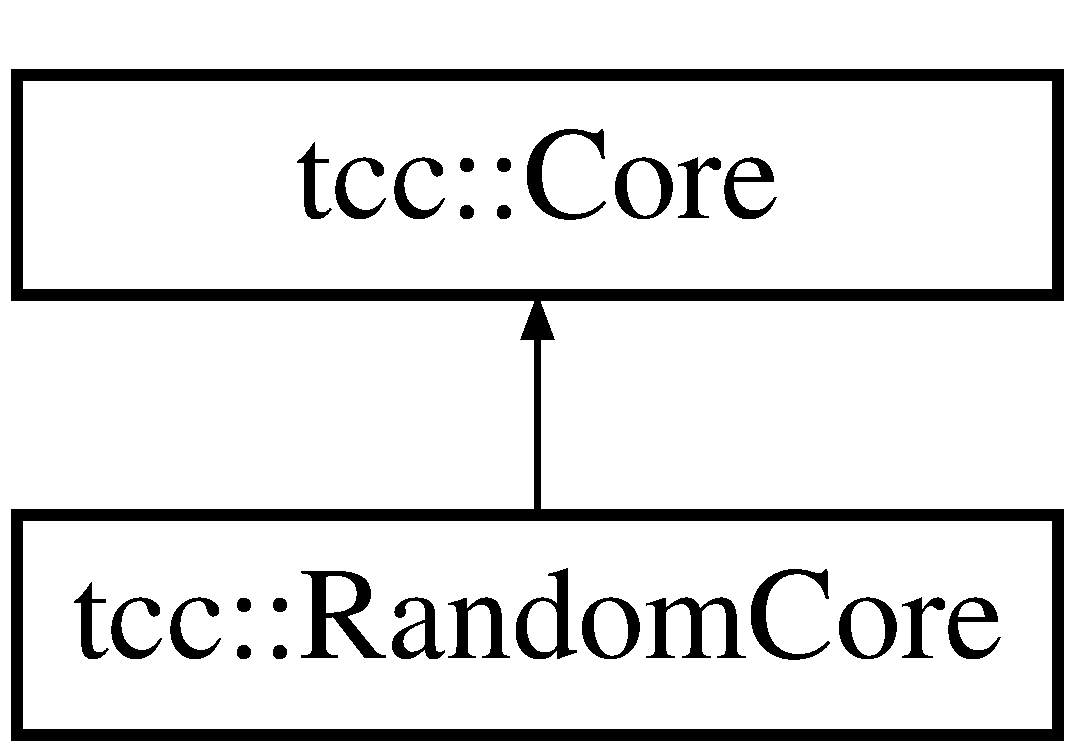
\includegraphics[height=2.000000cm]{classtcc_1_1_random_core}
\end{center}
\end{figure}


\subsection{Подробное описание}
Класс -\/ ядро для классификации \char`\"{}недоброжелательности\char`\"{} текста 

См. определение в файле Core.\+h строка 25



Объявления и описания членов класса находятся в файле\+:\begin{DoxyCompactItemize}
\item 
Cores/Core.\+h\end{DoxyCompactItemize}

%--- End generated contents ---

% Index
\backmatter
\newpage
\phantomsection
\clearemptydoublepage
\addcontentsline{toc}{chapter}{Алфавитный указатель}
\printindex

\end{document}
